\subsection{Learning Experiments}

\subsubsection{Model Architecture}

A base model architecture is used as a starting point for all learning experiments and is shown in Figure \ref{fig:architecture}. It consists of a head, a backbone, and a state estimator. The head consists of a configurable set of linear layers using the ReLU activation function. The backbone similarly is a configurable set of linear layers using the ReLU activation function that take as input the starting and goal position, along with any configuration parameters for the given dataset. These configuration parameters are tunable values that are indexed based on which robot setup was used to collect that data. A new configuration parameter is used for each time the robot has its tendons replaced. The state estimator is a configurable set of LSTM cells that take as input a horizon of motor feedback data. Specifically, experiments use current draw, encoder position, and encoder velocity for each motor. The output of the head is passed to one last linear layer without an activation layer. The output is then reshaped to be an $N\times 2$ vector where $N$ is the prediction horizon of the model. 

\begin{figure}[h]
    \centering
    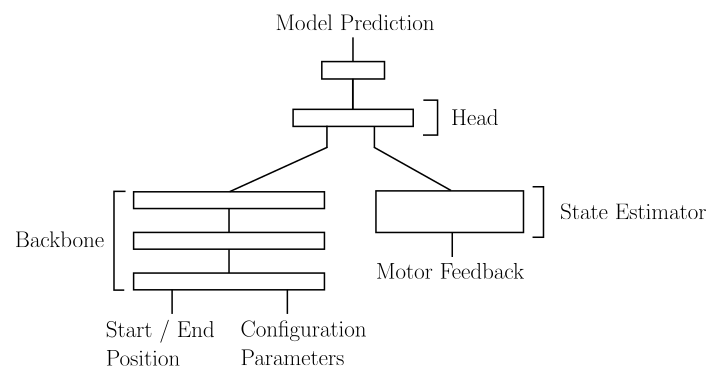
\includegraphics[width=0.8\textwidth]{images/architecture.png}
    \caption{Base model architecture for learning-experiments}
    \label{fig:architecture}
\end{figure}


\subsubsection{Training Parameters}
\label{sec:learning_baseline_description}
\paragraph{RMSE loss} is used for both training and comparing validation performance on a holdout dataset for each experiment (Equation \eqref{eq:rmse}). 

% Joint variable calculation 
\begin{equation}\label{eq:rmse}
    \operatorname{RMSE} = \sqrt{\frac{\displaystyle\sum_{i=1}^{N} ||y_{pred} - y_{gt}||^2 }{N}}
\end{equation}
where:
\begin{conditions}
y_\text{pred} & Predicted label from learned model \\
y_\text{gt} & Dataset label  \\
N & Number of items predicted \\
\end{conditions}

\paragraph{Constant training parameters} described in Table \ref{tab:training_parameters} are set and remained constant between all experiments. A runtime rate of \SI{1000}{Hz} for individual model calls is enforced for each trial to ensure that any model trained is capable of running in real time on the robot.  

\paragraph{Variable training parameters} described in Table \ref{tab:training_parameters} are varied through a series of experiments to find the optimal values for reducing validation loss. In each of these experiments (omitting the model architecture search trials), a baseline configuration is used as a comparison.

\begin{table}[h]
    \centering   
    \caption{Training parameters for learning experiments}
    \begin{tabular}{p{0.45\linewidth} | p{0.2\linewidth}}
        \textbf{Parameter} & \textbf{Value} \\
        \hline
        \multicolumn{2}{c}{Static Parameters} \\
        \hline
        Optimizer & Adam (default parameters) \\
        Learning rate & 0.001 \\
        Batch size & 512 \\
        Epochs & 1000 \\
        Early stopping & 10 \\
        \hline
        \multicolumn{2}{c}{Variable Parameters} \\
        \hline
        Feedback horizon & 1 - 300 \\
        Backbone layers & 1 - 3 \\
        Backbone layer size & 10 - 30 \\
        Head layers & 0 - 3 \\
        Head layer size & 0 - 50 \\
        LSTM layer size & 0 - 40 \\
        Configuration parameter size & 0 - 20 \\
        Data weights & Multiple \newline functions \\ 
    \end{tabular}
    \label{tab:training_parameters}
\end{table}

